\subsection{Test Drum Set and Hardware} \label{section:hardware}

For the development of the methods in this thesis, a standard drum set, a microphone, an external sound card and a laptop have been used. The used components are displayed in figure \ref{fig:components}.

\begin{SCfigure}[][h]
	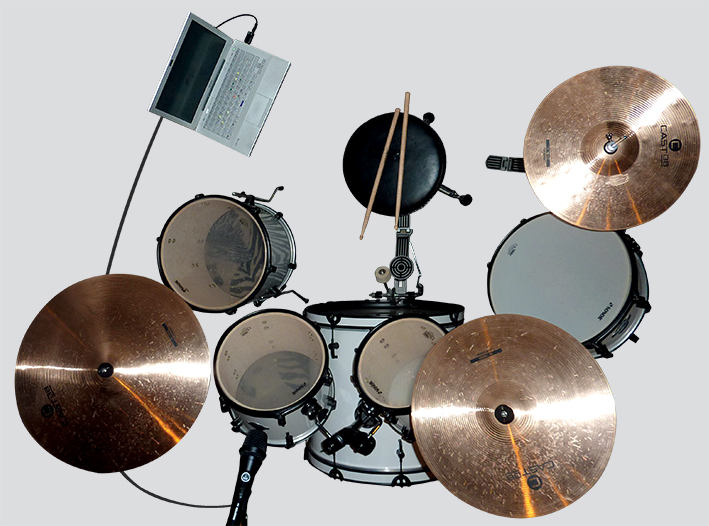
\includegraphics[width=10cm]{images/drumset/drumset_01.jpg}
	\caption{Hardware components 1. Basic drum set (Sonor SFX 11), 2. Maple leaf drumsticks, 3. Dynamic microphone (AKG P3 S), 4. External sound card (LogiLink 7.1), 5. Laptop (Sony VPCSB, 2.7 GHz, 8 GB RAM)}
	\label{fig:components} 
\end{SCfigure}

The used drum set is a basic Sonor SFX 11 drum set that consist of the following components:

\begin{itemize} 
	\item SMF 11 1816 BD WM Bass Drum 18" x 16"
	\item SMF 11 1455 SDW Snare Drum 14" x 5,5"
	\item SMF 11 1008 TT Tom Tom 10" x 8"
	\item SMF 11 1209 TT Tom Tom 12" x 9"
	\item SMF 11 1414 FT Floor Tom 14" x 14"
	\item CB8 Set 1 Cast B8 Cymbals (14" Hi-Hat, 16" Crash, 20" Ride)
	\item Maple wood drum sticks
\end{itemize}

The drum sound is recorded via a dynamic microphone (AKG P3 S) with an audio frequency bandwidth from	40 to 20000 Hz. It is linked to an external USB sound card (LogiLink 7.1) via xlr to 3.5 mm headphone jack. The software runs on an 2.7 GHz Sony VAIO Laptop with 8 GB RAM and the operation system Windows 7.
